%% Estructura principal para un reporte de Trabajos intersemanales CIRCAE %%
%% Autor: Edison Abado Ancco

\documentclass[a4paper]{article} %tamaño del papel y el tipo de transcripción que será IEEE
\usepackage[margin=2.8cm]{geometry}
%\usepackage[total={6.5in,10in},left=1in,top=0.5in,includehead,includefoot]{geometry}
\usepackage[utf8]{inputenc} %el tipo de codificación que incluye símbolos como la tilde
\usepackage[spanish]{babel} % hacemos que nuestro documentación vaya en español
\usepackage{cite} % citas bibliográficas
\usepackage{graphicx} %gráficos, usaremos solo .jpg o .png con estándares que ya veremos
%\usepackage{subfigure} %usar subfiguras
\usepackage{url} %agregar direcciones url
\usepackage{amsmath} %expresiones matemáticas
\newtheorem{teor}{Teorema}[section] %definimos la enumeración de Teoremas usando la etiqueta \begin{teor} ... \end{teor} para los ejemplos, podemos darle etiquetas para referenciarlas a lo largo del texto
\newtheorem{ejem}{Ejemplo}[section] %definimos la enumeración de Ejemplos usando la etiqueta \begin{ejem} ... \end{ejem} para los ejemplos, podemos darle etiquetas para referenciarlas a lo largo del texto
\newtheorem{exper}{Experimento}[section] %definimos la enumeración de Ejemplos usando la etiqueta \begin{exper} ... \end{exper} para los Experimentos, podemos darle etiquetas para referenciarlas a lo largo del texto
\usepackage{setspace} %LA usamos para asignar el interlineado
%%%%%%% settings para incluir codigo fuente en cualquier lenguaje
\usepackage{listings} %comenzamos la configuración de nuestras lineas de codigo que se incluirá de ser necesario en el documento
\usepackage[usenames]{color} %seteamos el uso de nombre y color
\definecolor{gray97}{gray}{.97}%definimos nombre y color
\usepackage{textcomp}
\usepackage{tikz,bm}
\usetikzlibrary{calc, positioning, shapes, backgrounds, fit, arrows}
\usepackage{tikz,bm}
\usepackage[raggedrightboxes]{ragged2e}
\usepackage{pgf-spectra}

\usepackage{siunitx}

\usepackage{contour}
\lstset{
	frame=Ltb,
	framerule=1pt,
	framextopmargin=5pt, %margen de arriba
	framexbottommargin=5pt, %margen de abajo
	framexleftmargin= -2pt, %separacion del margen izquierdo
	framesep=2pt,
	rulesep=0.2pt,
	backgroundcolor=\color{gray97},
	rulesepcolor=,
	tabsize=4,
	rulecolor=\color[RGB]{106, 182, 217}, %AZUL
	upquote=true,
	aboveskip={1.5\baselineskip}, %despues de la linea de texto
	columns=fixed,
	showstringspaces=false,
	extendedchars=true,
	breaklines=true,
	prebreak = \raisebox{0ex}[0ex][0ex]{\ensuremath{\hookleftarrow}},
	showtabs=false,
	showspaces=false,
	showstringspaces=false,
	basicstyle=\scriptsize\ttfamily\color[RGB]{39, 100, 46}, %Numeros de lineas, simbolos, puntos y coma y demas
	identifierstyle=\ttfamily\color[RGB]{56, 140, 189}, %variables
	commentstyle=\color[RGB]{62, 179, 101}, %comentarios
	stringstyle=\color[RGB]{247, 165, 42}, %impresiones
	keywordstyle=\bfseries\color[RGB]{237, 118, 150}, %funciones
	%
	numbers=left,
	numbersep=-7pt, %separacion del numero
	numberstyle=\tiny,
	numberfirstline = false,
	breaklines=true,
}
\usepackage{graphicx}
\usepackage[colorinlistoftodos]{todonotes}
\usepackage{enumitem}
%%%%%%%
\providecommand{\keywords}[1]{\textbf{\textit{Términos Clave---}} #1}

\usepackage{hyperref}
\usepackage{wrapfig}
\usepackage{caption}
\usepackage{subcaption}

\begin{document}
\spacing{0.9} %definimos un interlineado de 0.9 para todo el documento

\begin{titlepage}
	\newcommand{\HRule}{\rule{\linewidth}{0.5mm}} 
	\center
	\textsc{\LARGE  Universidad Nacional de San \\[0.2cm] Antonio Abad del Cusco}\\[1.5cm] 
	
\includegraphics[width=4cm]{IMAGENES/escudo}\\[1cm]
	\textsc{\Large Facultad de Ingeniería Eléctrica, \\ Electrónica, Informática y Mecánica}\\[0.5cm] 
	\textsc{\large Escuela Profesional de Ingeniería Electrónica}\\[0.5cm]
	\textsc{\Large Laboratorio de Circuitos electrónicos I}\\[0.5cm]
	\HRule \\[0.4cm]
	{ \huge \bfseries Rectificadores de media onda y onda completa}\\[0.4cm] 
	\HRule \\[1.5cm]
	\begin{minipage}{\textwidth}
		\center 
		
		\emph{Profesor} \\
		Ing. Juan Pablo \textsc{Vizcardo Zuniga} \\[1cm]
		
		\begin{tabular}{lll}
			\emph{Alumno} & \emph{Código} & \emph{Correo}\\
			Edison \textsc{Abado Ancco } & 145012 & 145012@unsaac.edu.pe\\
			
		\end{tabular}
	\end{minipage}\\[2cm]
	\today
\end{titlepage}


%\tableofcontents indice bloqueado xD

\newpage


\begin{abstract}
	Un diodo es un componente electrónico formado por la unión PN, y tiene la funcionalidad que permite la circulación de la corriente eléctrica a través de él en un solo sentido, bloqueando el paso si la corriente circula en sentido contrario, esto hace que el diodo tenga dos posibles posiciones: una a favor de la corriente (polarización directa) y otra en contra de la corriente (polarización inversa). Los rectificadores de onda son circuitos con diodos que permiten convertir la corriente alterna en corriente continua.
	Atendiendo al tipo de rectificación, pueden ser de media onda, cuando solo se utiliza uno de los semiciclos de la corriente, o de onda completa, donde ambos semiciclos son aprovechados.
\end{abstract}
	
\newpage
	
\section{Obtenga las siguientes relaciones teóricas para el rectificador de media onda}
\label{concepto}



\subsection{Valor medio y eficaz de Tensión}

El valor medio desde el punto de vista matemático es la integral de una determinada señal en un periodo dividida sobre el mismo periodo:

\begin{equation}
	v_m = \frac{1}{T} \int_{0}^{T} f(t) dt
\end{equation}

El valor eficaz o rms de una señal periódica de voltaje o de corriente es aquel que produce la misma potencia media que una señal dc sobre carga resistiva. La función matemática que define el valor eficaz de una señal es la siguiente:

\begin{equation}
	v_{ef} = \sqrt{\frac{1}{T} \int_{0}^{T} f^2 (t) dt}
\end{equation}

Dado que para una onda senoidal, y una rectificación de onda tendrá la forma: 

\begin{tikzpicture} 
	\draw (0,0) -- (12,0);
	\draw (0.2,1)node[left,font=\tiny] {$v_p$} -- (12,1);
	\draw (0.2,-1)node[left,font=\tiny] {$-v_p$} -- (12,-1); 
	\foreach \x in {0,0.5,...,12}{
		\draw (\x,-0.2)node [below,font=\tiny,] {\x} -- (\x,0.2) ;
	}
	\draw[ultra thick, red] (0,0) sin (1,1);    %% the real business in this line
	\draw[ultra thick, red] (1,1) cos (2,0);    %% the real business in this line
	\draw[ultra thick, red] (2,0) sin (4,0);
	\draw[ultra thick, blue] (4,0) sin (5,1);    %% the real business in this line
	\draw[ultra thick, blue] (5,1) cos (6,0);    %% the real business in this line
	\draw[ultra thick, blue] (6,0) sin (8,0);
	\draw[ultra thick, green] (8,0) sin (9,1);    %% the real business in this line
	\draw[ultra thick, green] (9,1) cos (10,0);    %% the real business in this line
	\draw[ultra thick, green] (10,0) sin (12,0);
	%% the real business in this line
\end{tikzpicture}

su ecuación es:

\begin{equation}
	f(t) = \begin{cases}
		v_p sin(wt) & 0 \leq t \leq \frac{T}{2} \\
		0 & \frac{T}{2} \leq t \leq T
	\end{cases}
\end{equation}

El valor medio de la tensión de carga $v_m$ está dado por:

\begin{equation}
	v_{m} = \frac{v_p}{\pi}
\end{equation}

El valor eficaz $v_{ef}$ estará dado por:

\begin{equation}
	v_{ef} = \frac{v_p}{2}
\end{equation}

Cuando se considere la tensión umbral del diodo $V_k$, y esta sea $v_k \ll v_m$, entonces la tensión promedio estaará dado por:

\begin{equation}
	v_{m} = \frac{v_p - v_k}{\pi}
\end{equation}

El valor eficaz $v_{ef}$ estará dado por:

\begin{equation}
	v_{ef} = \frac{v_p - v_k}{2}
\end{equation}

\subsection{Valor medio y eficaz de Corriente}

Por la ley de Ohm, la corriente media está dada por:

\begin{equation}
	i_{m} = \frac{v_{m}}{R_L}
\end{equation}

Y la corriente eficaz estará dado por:

\begin{equation}
	i_{ef} = \frac{v_{ef}}{R_L}
\end{equation}

\section{Obtenga las siguientes relaciones teóricas para el rectificador de onda completa}

\begin{tikzpicture} 
	\draw (0,0) -- (12,0);
	\draw (0.2,1)node[left,font=\tiny] {$v_p$} -- (12,1);
	\draw (0.2,-1)node[left,font=\tiny] {$-v_p$} -- (12,-1); 
	\foreach \x in {0,0.5,...,12}{
		\draw (\x,-0.2)node [below,font=\tiny,] {\x} -- (\x,0.2) ;
	}
	\draw[ultra thick, red] (0,0) sin (1,1);    %% the real business in this line
	\draw[ultra thick, red] (1,1) cos (2,0);    %% the real business in this line
	\draw[ultra thick, red] (2,0) sin (3,1);
	\draw[ultra thick, red] (3,1) cos (4,0);
	\draw[ultra thick, blue] (4,0) sin (5,1);    %% the real business in this line
	\draw[ultra thick, blue] (5,1) cos (6,0);    %% the real business in this line
	\draw[ultra thick, blue] (6,0) sin (7,1);
	\draw[ultra thick, blue] (7,1) cos (8,0);
	\draw[ultra thick, green] (8,0) sin (9,1);    %% the real business in this line
	\draw[ultra thick, green] (9,1) cos (10,0);    %% the real business in this line
	\draw[ultra thick, green] (10,0) sin (11,1);
	\draw[ultra thick, green] (11,1) cos (12,0);
	%% the real business in this line
\end{tikzpicture}

cuya ecuación es:

\begin{equation}
	v(t) = |v_p sin(wt)|
\end{equation}

\subsection{Valor medio y eficaz de Tensión}

El valor medio de la tensión de carga $v_0$ está dado por:

\begin{equation}
	v_m = 2\frac{v_p}{\pi}
\end{equation}

El valor eficaz $v_{ef}$ estará dado por:

\begin{equation}
	v_{ef} = \frac{v_p}{\sqrt{2}}
\end{equation}


Cuando se considere la tensión umbral del diodo $V_k$, y esta sea $v_k \ll v_m$, entonces la tensión promedio estaará dado por:

\begin{equation}
	v_m = 2\frac{v_p - 2v_k}{\pi}
\end{equation}

El valor eficaz $v_{ef}$ estará dado por:

\begin{equation}
	v_{ef} = \frac{v_p - 2v_k}{\sqrt{2}}
\end{equation}


\subsection{Valor medio y eficaz de Corriente}

Por la ley de Ohm, la corriente media está dada por:

\begin{equation}
	\overline{i_{m}} = 2\frac{\overline{v_{m}}}{R_L}
\end{equation}

Y la corriente eficaz estará dado por:

\begin{equation}
	i_{ef} = 2\frac{v_{ef}}{R_L}
\end{equation}

\section{Armar el siguiente circuito para encontrar el voltaje umbral del diodo por defecto de LTSpice}

Para poder ver el voltaje por defecto del diodo, nos fijamos en la figura \eqref{fig1}, donde nos muestra una tensión $v_k = 0.7177V$

\begin{figure} %Comenzar la figura
	\centering %hacemos que la imagen en cuestion esté centrada, si guera de 5 o 6 cm, esta se vea bien
	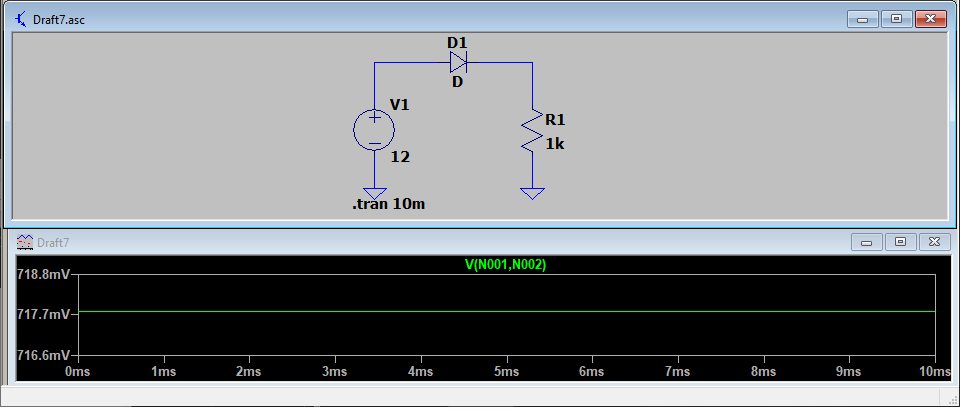
\includegraphics[scale=0.5]{IMAGENES/fig1} %incluimos la imagen con una característica especial: la medida definida en centímetros e incluimos la ruta de imagen sin especificar la extensión de la imagen (solo usaremos .png y .jpg)
	\caption{Tensión umbral por defecto del diodo el LTSpice} %La descripción de la imagen, ser concisos
	\label{fig1} %La etiqueta usada para poder referenciarla desde cualquier parte del texto como se hizo con /eqref{img1}
\end{figure} %finalizamos la figura

\section{Encontrar el voltaje umbral del diodo 1N4004}

Una vez agregado la librería del diodo, la incluimos en nuestro esquemático y medimos la tensión entre anodo y cátodo. Con ello podemos encontrar una tensión umbral $v_k = 0.635V$ como se muestra en la figura \eqref{fig2}

\begin{figure} %Comenzar la figura
	\centering %hacemos que la imagen en cuestion esté centrada, si guera de 5 o 6 cm, esta se vea bien
	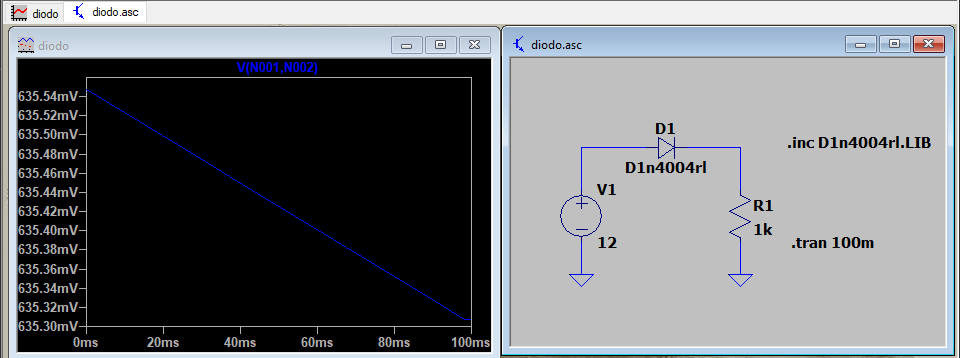
\includegraphics[scale=0.5]{IMAGENES/fig2} %incluimos la imagen con una característica especial: la medida definida en centímetros e incluimos la ruta de imagen sin especificar la extensión de la imagen (solo usaremos .png y .jpg)
	\caption{Tensión umbral del diodo D1n4004rl, en la imagen se muestra su valor con respecto al tiempo, pero coonsiderese la escala.} %La descripción de la imagen, ser concisos
	\label{fig2} %La etiqueta usada para poder referenciarla desde cualquier parte del texto como se hizo con /eqref{img1}
\end{figure} %finalizamos la figura

\section{Para el siguiente circuito rectificador de media onda}

Dado el circuito de la figura \eqref{fig2.1}, podemos hallar los valores pedidos usando la directiva \texttt{.meas} como se muestra en la figura \eqref{fig3}

\begin{figure} %Comenzar la figura
	\centering %hacemos que la imagen en cuestion esté centrada, si guera de 5 o 6 cm, esta se vea bien
	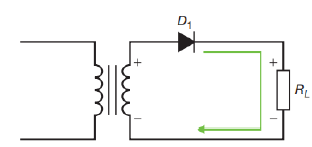
\includegraphics[scale=0.8]{IMAGENES/fig2.1} %incluimos la imagen con una característica especial: la medida definida en centímetros e incluimos la ruta de imagen sin especificar la extensión de la imagen (solo usaremos .png y .jpg)
	\caption{Enunciado de la pregunta 5.} %La descripción de la imagen, ser concisos
	\label{fig2.1} %La etiqueta usada para poder referenciarla desde cualquier parte del texto como se hizo con /eqref{img1}
\end{figure} %finalizamos la figura

\begin{figure} %Comenzar la figura
	\centering %hacemos que la imagen en cuestion esté centrada, si guera de 5 o 6 cm, esta se vea bien
	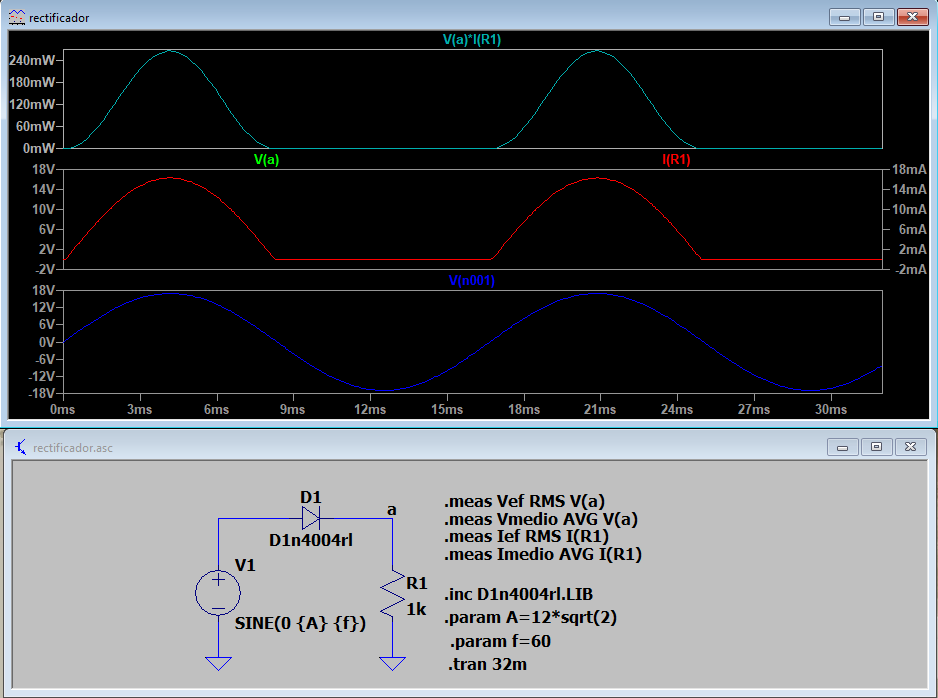
\includegraphics[scale=0.5]{IMAGENES/fig3} %incluimos la imagen con una característica especial: la medida definida en centímetros e incluimos la ruta de imagen sin especificar la extensión de la imagen (solo usaremos .png y .jpg)
	\caption{Gráfico del rectificador de media onda para la pregunta 5, usando la directiva \texttt{.meas}. Se puede ver valores de Tensión, corriente y \textbf{potencia}.} %La descripción de la imagen, ser concisos
	\label{fig3} %La etiqueta usada para poder referenciarla desde cualquier parte del texto como se hizo con /eqref{img1}
\end{figure} %finalizamos la figura

Viendo en la ventana de \texttt{error Log} veremos lo siguiente: 

\begin{itemize}
	\item $v_{L,m,lab}$: AVG(v(a))=6.86744 FROM 0 TO 0.032
	\item $v_{L,ef,lab}$: RMS(v(a))=7.78817 FROM 0 TO 0.032
	\item $i_{L,ef,lab}$: RMS(i(r1))=0.119818 FROM 0 TO 0.032
	\item $i_{L,m,lab}$: AVG(i(r1))=0.105653 FROM 0 TO 0.032
\end{itemize}

Todos estos valores están dados en el S.I. de unidades.

\subsection{Análisis teórico}
Se tiene como entrada una señal de $v_i = V_{i_{RMS}}\sqrt{2}sin(2 \pi f t)$, como dato tenemos $V_{i_{RMS}} = 12V$ y $f=60Hz$, para los valores en la carga tendríamos lo siguiente:

\begin{align}
	v_{L,m, teorico} = & 2\frac{ V_{i_{RMS}}\sqrt{2} - 2v_k}{\pi} = 2 \left(\frac{9\sqrt{2} - 2(0.635)}{\pi}\right) = 7.29433 V \\
	v_{L,ef, teorico} = & \frac{ V_{i_{RMS}}\sqrt{2} - 2v_k}{\sqrt{2}} = \frac{9\sqrt{2} - 2(0.635)}{\sqrt{2}} = 8.10197V \\
	i_{L,ef, teorico} = & \frac{v_ {L,ef, teorico}}{R_L} = \frac{8.10197}{65} = 8.16778 mA \\
	i_{L,m,teorico} = & \frac{v_{L,m, teorico}}{R_R} = \frac{7.29433}{65} = 5.19977mA
\end{align}
Por lo que el error experimental con respecto al teórico está dado por:

\begin{align}
	\varepsilon_{v_{L,m}} \% = & \left|\frac{v_{L,m,lab} - v_{L,m,teorico}}{v_{L,m,teorico}} \right| = \left| \frac{5.19977 - 5.30879}{5.19977} *100 \right|= 2.0966 \% \\
	\varepsilon_{v_{L,ef}} \% = & \left|\frac{v_{L,ef,lab} - v_{L,ef,teorico}}{v_{L,ef,teorico}} \right| = \left| \frac{8.24671 - 8.16778}{8.16778} *100 \right|= 0.96636 \% \\
	\varepsilon_{i_{L,ef}} \% = & \left|\frac{i_{L,ef,lab} - i_{L,ef,teorico}}{i_{L,ef,teorico}} \right| = \left| \frac{8.24671m - 8.16778m}{8.16778m} *100 \right|= 0.96636 \% \\
	\varepsilon_{i_{L,m}} \% = & \left|\frac{i_{L,m,lab} - i_{L,m,teorico}}{i_{L,m,teorico}} \right| = \left| \frac{5.19977m - 5.30879m}{5.19977m} *100 \right|= 2.0966 \%
\end{align}

\section{Para el circuito anterior, invertir el sentido del diodo, visualizar la forma de onda de voltaje en la carga.}

Para ello tans olo invertimos el diodo, y simulamos en el mismo circuito. El resultado se verá en la figura \eqref{fig4}

\begin{figure} %Comenzar la figura
	\centering %hacemos que la imagen en cuestion esté centrada, si guera de 5 o 6 cm, esta se vea bien
	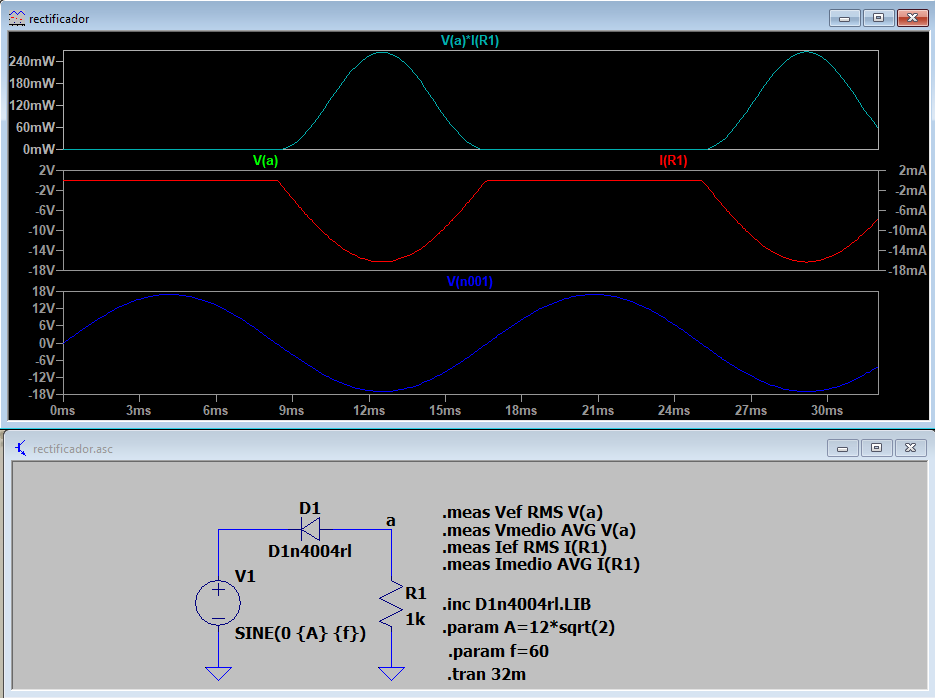
\includegraphics[scale=0.5]{IMAGENES/fig4} %incluimos la imagen con una característica especial: la medida definida en centímetros e incluimos la ruta de imagen sin especificar la extensión de la imagen (solo usaremos .png y .jpg)
	\caption{Gráfico del rectificador de media onda con el diodo invertido para la pregunta 6, usando la directiva \texttt{.meas}. Se puede ver valores de Tensión, corriente y \textbf{potencia}.} %La descripción de la imagen, ser concisos
	\label{fig4} %La etiqueta usada para poder referenciarla desde cualquier parte del texto como se hizo con /eqref{img1}
\end{figure} %finalizamos la figura

\section{Para el circuito anterior, variar la frecuencia de la señal alterna por 1KHz y luego 1MHz y visualizar las formas de onda del voltaje en la carga.}

Para ello, tan solo variamos la frecuencia, y para que las ventanas de visualización muestren cláramente la onda, variamos el \texttt{Stop Time} de nuestra vetana de configuración de la simulación. Para este caso, para $1KHz$ se puso $2m$ segundos (ver figura \eqref{fig5}), y para $1MHz$ se puso $1u$ segundo (ver figura \eqref{fig6}). Se puede notar que para una señal algo grande de $1MHz$ se puede ver que la señal de salida se deforma un poco, esto debido al diodo que se está usando, que está diseñado para tensiones altas, pero frecuencias bajas.

\begin{figure} %Comenzar la figura
	\centering %hacemos que la imagen en cuestion esté centrada, si guera de 5 o 6 cm, esta se vea bien
	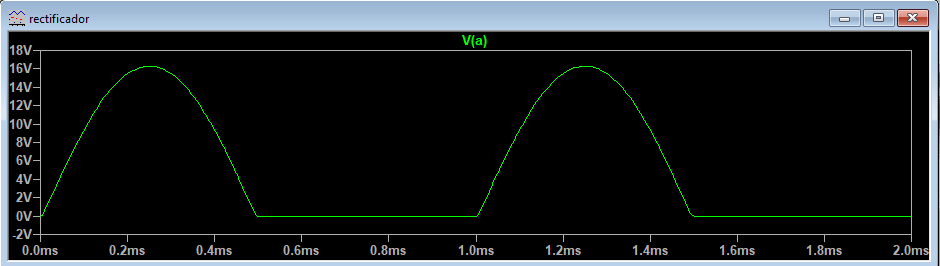
\includegraphics[scale=0.5]{IMAGENES/fig5} %incluimos la imagen con una característica especial: la medida definida en centímetros e incluimos la ruta de imagen sin especificar la extensión de la imagen (solo usaremos .png y .jpg)
	\caption{Gráfico de tensión para $1KHz$ con \texttt{Stop Time} de $2m$ segundos.} %La descripción de la imagen, ser concisos
	\label{fig5} %La etiqueta usada para poder referenciarla desde cualquier parte del texto como se hizo con /eqref{img1}
\end{figure} %finalizamos la figura

\begin{figure} %Comenzar la figura
	\centering %hacemos que la imagen en cuestion esté centrada, si guera de 5 o 6 cm, esta se vea bien
	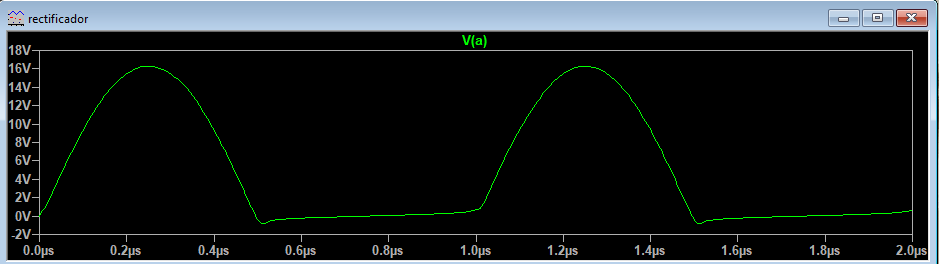
\includegraphics[scale=0.5]{IMAGENES/fig6} %incluimos la imagen con una característica especial: la medida definida en centímetros e incluimos la ruta de imagen sin especificar la extensión de la imagen (solo usaremos .png y .jpg)
	\caption{Gráfico de tensión para $1MHz$ con \texttt{Stop Time} de $2u$ segundos.} %La descripción de la imagen, ser concisos
	\label{fig6} %La etiqueta usada para poder referenciarla desde cualquier parte del texto como se hizo con /eqref{img1}
\end{figure} %finalizamos la figura

\section{Para el siguiente circuito rectificador de onda completa}

Vemos el circuito de la figura \eqref{fig7}, para ello se asume un transformador de 220V / 9V (60Hz), 4 diodos 1N4004 y una carga RL de 65 ohm.

\begin{figure} %Comenzar la figura
	\centering %hacemos que la imagen en cuestion esté centrada, si guera de 5 o 6 cm, esta se vea bien
	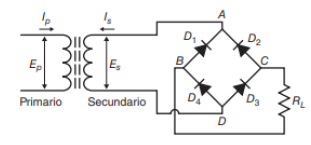
\includegraphics[scale=0.8]{IMAGENES/fig7} %incluimos la imagen con una característica especial: la medida definida en centímetros e incluimos la ruta de imagen sin especificar la extensión de la imagen (solo usaremos .png y .jpg)
	\caption{Circuito de onda completa para el enunciado 8.} %La descripción de la imagen, ser concisos
	\label{fig7} %La etiqueta usada para poder referenciarla desde cualquier parte del texto como se hizo con /eqref{img1}
\end{figure} %finalizamos la figura

Armamos el circuito, usamos las directivas .meas para los valores pedidos, seteamos los parámetros de la simulación, separamos ventanas, y obtendremos el gráfico de la figura \eqref{fig8}

\begin{figure} %Comenzar la figura
	\centering %hacemos que la imagen en cuestion esté centrada, si guera de 5 o 6 cm, esta se vea bien
	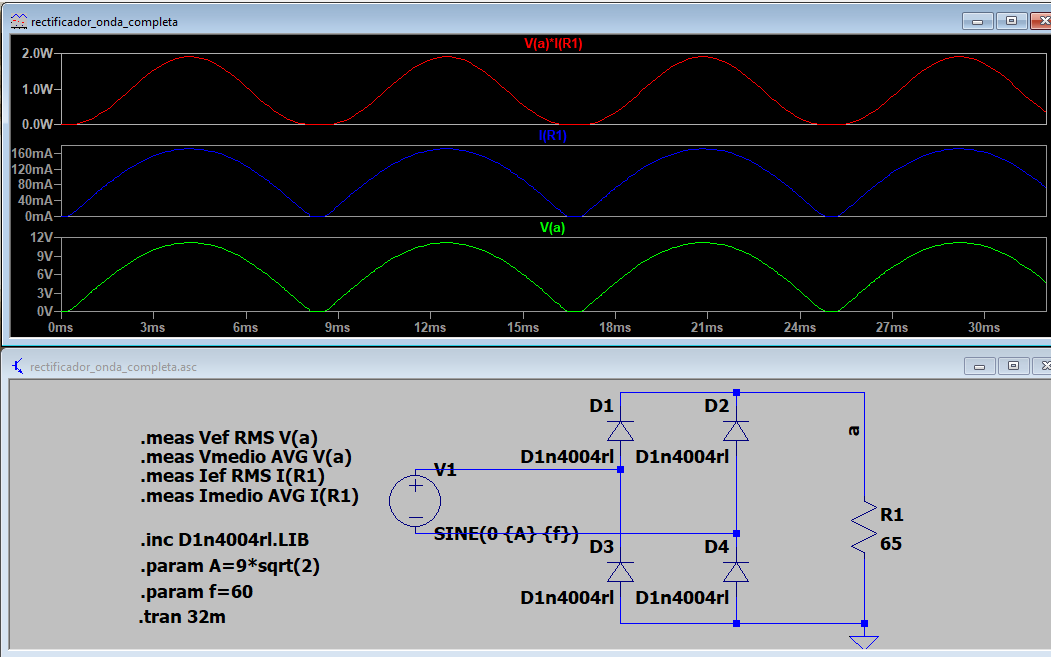
\includegraphics[scale=0.5]{IMAGENES/fig8} %incluimos la imagen con una característica especial: la medida definida en centímetros e incluimos la ruta de imagen sin especificar la extensión de la imagen (solo usaremos .png y .jpg)
	\caption{Simulación de un circuito de Onda completa.} %La descripción de la imagen, ser concisos
	\label{fig8} %La etiqueta usada para poder referenciarla desde cualquier parte del texto como se hizo con /eqref{img1}
\end{figure} %finalizamos la figura

Para hallar los valores que pide el enunciado, debido a que usamos la directiva \texttt{.meas}, tan solo vemos la ventana de \texttt{SPICE Error Log}, y vemos los valores que muestra.

\begin{itemize}
	\item $v{vmedio}$: AVG(v(a))=6.86744 FROM 0 TO 0.032
	\item $v_{ef}$: RMS(v(a))=7.78817 FROM 0 TO 0.032
	\item $i_{ef}$: RMS(i(r1))=0.119818 FROM 0 TO 0.032
	\item $i_{medio}$: AVG(i(r1))=0.105653 FROM 0 TO 0.032
\end{itemize}

\subsection{Análisis teórico}
Se tiene como entrada una señal de $v_i = V_{i_{RMS}}\sqrt{2}sin(2 \pi f t)$, como dato tenemos $V_{i_{RMS}} = 9V$ y $f=60Hz$, $R_L = 65 \Omega$ para los valores en la carga tendríamos lo siguiente:

\begin{align}
	v_{L,m, teorico} = & 2\frac{  V_{i_{RMS}}\sqrt{2} - 2v_k}{\pi} = 2 \frac{12\sqrt{2} - (2)0.635}{\pi} = 7.2943 V \\
	v_{L,ef, teorico} = & \frac{ V_{i_{RMS}}\sqrt{2} - 2v_k}{\sqrt{2}} = \frac{9\sqrt{2} - (2)0.635}{\sqrt{2}} = 8.4838V \\
	i_{L,ef, teorico} = & \frac{v_ {L,ef, teorico}}{R_L} = \frac{8.4838}{65} = 130.52 mA \\
	i_{L,m,teorico} = & \frac{v_{L,m, teorico}}{R_R} = \frac{7.2943}{65} = 112.22mA
\end{align}
Por lo que el error experimental con respecto al teórico está dado por:

\begin{align}
	\varepsilon_{v_{L,m}} \% = & \left|\frac{v_{L,m,lab} - v_{L,m,teorico}}{v_{L,m,teorico}} \right| = \left| \frac{6.86744 - 7.2943}{7.2943} *100 \right|= 5.8524 \% \\
	\varepsilon_{v_{L,ef}} \% = & \left|\frac{v_{L,ef,lab} - v_{L,ef,teorico}}{v_{L,ef,teorico}} \right| = \left| \frac{7.78817 - 8.4838}{8.4838} *100 \right|= 8.1996 \% \\
	\varepsilon_{i_{L,ef}} \% = & \left|\frac{i_{L,ef,lab} - i_{L,ef,teorico}}{i_{L,ef,teorico}} \right| = \left| \frac{119.818m - 130.52m}{130.52m} *100 \right|= 8.2056 \% \\
	\varepsilon_{i_{L,m}} \% = & \left|\frac{i_{L,m,lab} - i_{L,m,teorico}}{i_{L,m,teorico}} \right| = \left| \frac{105.653m - 112.22m}{112.22m} *100 \right|= 5.9410 \%
\end{align}

Notamos que el error es más significativo que en el ejemplo 1, debido a que la tensión pico de la fuente tuvo una disminución.

	%%%%%%%%%%%%%%%%%%%%%%%%%%%%%%%%%%%%%%%%%%%%%%%
	%%%%%
	%%%%%   BIBLIOGRAFÍA    %%%%%%%%%%%%%%%%%%%%%% No tenemos :'v sad
	%%%%%
	%%%%%%%%%%%%%%%%%%%%%%%%%%%%%%%%%%%%%%%%%%%%%%%
	
% Este es un comentario xD
%Probando git probando y probando	
	
%	\bibliographystyle{ieeetr}
%	\bibliography{bibliografia}
	
\end{document}

